The original dataset is composed by 4 tables in CSV fomat: \textit{pos.csv}, \textit{rental.csv}, \textit{user.csv}, \textit{device.csv}. This dataset is a subset of another dataset with some sensitive data dropped (like user name or email) and positions manumit in order to protect proprietary data. Although this dataset is only a subset of the proprietary data, the positions amount is really huge and it weighs about 2GB. 

The \textit{pos.csv} table contains all the positions, characterized by latitude, longitude, speed, timestamp and a device id used to join with \textit{device.csv} table. The \textit{device.csv} and \textit{user.csv} tables contain the kilometres travelled respectively by a scooter and by a user. At last, the \textit{rental.csv} table contains the start position and end position in couple of longitude and latitude of the rental trajectories with related start and stop timestamps, and all the ids used to join the other tables with this one (dataset diagram in figure \ref{original-dataset-diagram}). The figure \ref{fig:starting-point} shows all positions in the two Italy cities.

\begin{figure*}[bt]
	\centering
	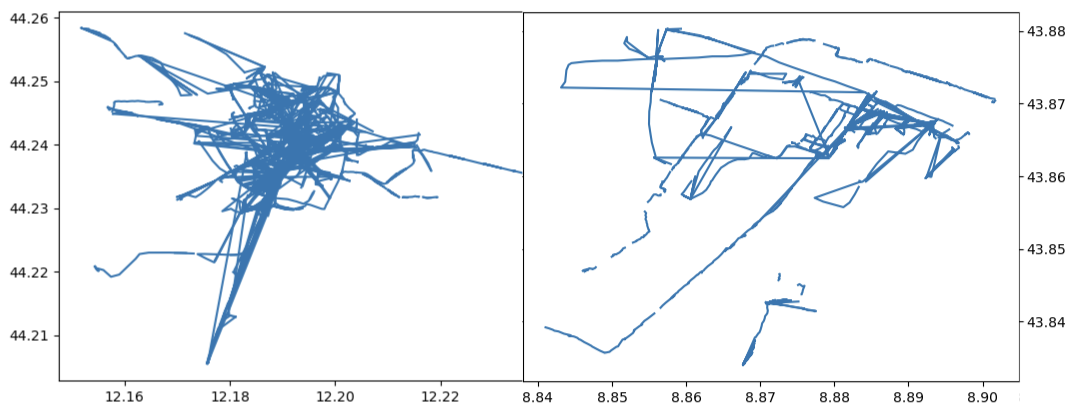
\includegraphics[width=\textwidth]{starting-point}
	\caption{Trajectories without clustering in 2 Italy cities}
	\label{fig:starting-point}
\end{figure*}

The first thing that I noticed is that the dataset is not built very well and I would have the positions in relation with its rental and not with its device. Therefore I preferred to lose some positions saved by different devices, I joined the position and rental tables through their ids and I filtered it in order to obtain only the positions that belongs in the range of rental start-end time (figure \ref{generated-dataset-diagram}). This operation was really tricky because the total amount of data is huge and I had to use optimized functions based on database join algorithms and chunks management to be able to handle these data in shot time. At last, the resulting table has been sorted for rental id, position id and timestamp, in order to have everything ready to perform plot representation and some feature analysis.

\begin{figure}[bt]
	\centering
	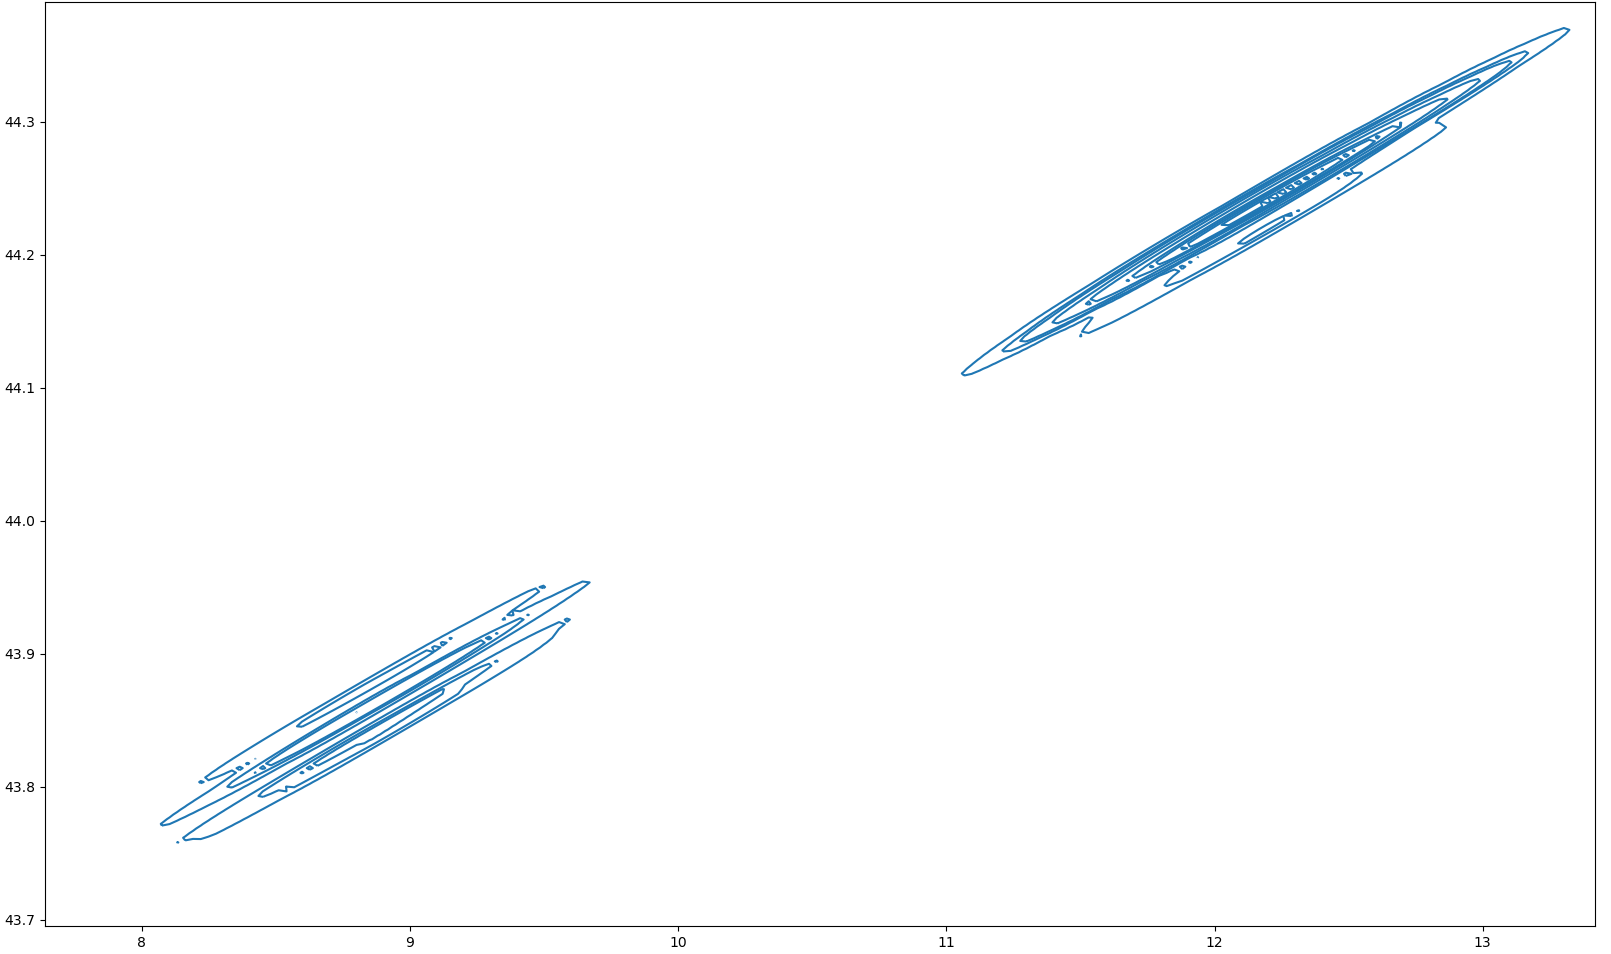
\includegraphics[width=\columnwidth]{pos-distributions}
	\caption{Distribution of positions: mainly developed in 2 Italy cities}
	\label{fig:pos-distributions}
\end{figure}

After that, I performed some analysis on features. I studied their distribution (figure \ref{fig:pos-distributions}) and I started to think how could be possible to group or divide positions. In particular I learnt that two trajectories can be similar in shape and can be divided in time. It means that a sequence of positions, a trajectory, can be similar to another one, evaluating his shape appearance and location in the geographical map, and therefore his sequence of their geographical coordinates. On the other hand, a trajectory can be different to another one if there is a temporal space between each other. The starting assumption of this analysis is that all positions belong to a rental, it means that starting from how data are constructed, I assume that a trajectory is the sequence of positions sorted in time that belong to the same rental (figure \ref{fig:rental-plot}). 

\begin{figure*}[bt]
	\centering
	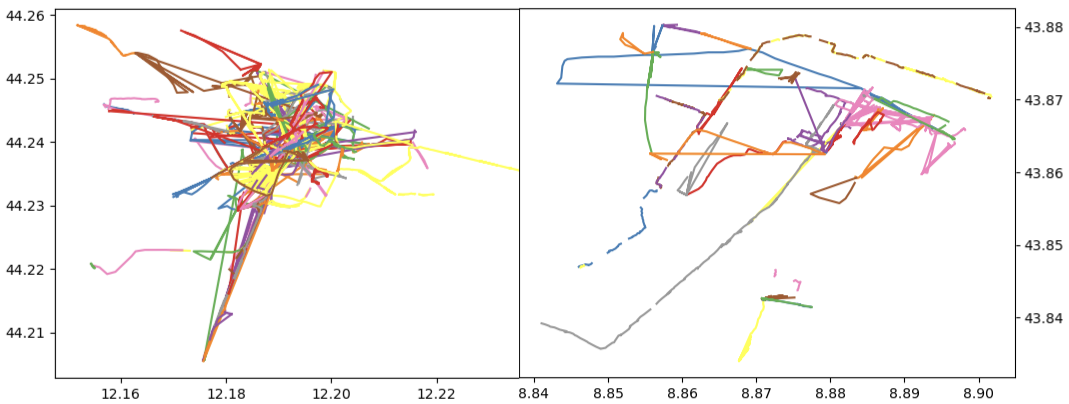
\includegraphics[width=\textwidth]{rental-plot}
	\caption{Trajectories belonging rentals}
	\label{fig:rental-plot}
\end{figure*}

\begin{table}
	\centering
	\caption{Number of features and samples of generated dataset}
	\begin{tabular}{ l r r }
		\hline
		Dataset & Samples & Features \\ \hline
		rental & 14826 & 10 \\ 
		pos & 817076 & 18 \\ 
		merge & 817076 & 18 \\
		dataset & 14826 & 13 \\
		partition city 1 & 608251 & 18 \\
		partition city 2 & 202795 & 18 \\ \hline
	\end{tabular}
\end{table}

As result I implemented 3 different clustering heuristics performed in a systematic and statistical way on the entire sequence of positions:
\begin{itemize}
	\item \textbf{timedelta heuristic}: considers that a trajectory of a rental can be divided in a sequence of trajectories if the time gap between a position and previous one exceeds a \textit{timedelta} value. First of all I calculated the time gaps for each set of positions grouping in rental: 
	\begin{align}
		TIMEGAPS = \{p.time - p[-1].time \mid \forall p \in POS \}
	\end{align}
	where \verb|p[-1]| is the previous position and the field \verb|.time| is the position timestamp. The \textit{timedelta} value can be assigned or can be automatically calculated. To calculate automatically the timedelta value I plotted the timegaps distribution and I exploited the statistical empirical rule to cover a percentage of timegaps distribution. In this case I take all the left tail of the distribution and the $43\%$ of the right one, and that ones that remains outside are the positions candidates that divide a trajectory from another one. This operation has been performed for each rental positions in order to obtain a set of sub-trajectories of rental trajectory.
	\item \textbf{spreaddelta heuristic}: considers that a rental trajectory can be considered similar to another one if they spread a similar amount of area. I calculate the spread area for each rental trajectory in the following way: 
	\begin{align}
		SPREADS = \{max(t) - min(t) \mid \forall t \in TRAJ \}
	\end{align}
	where \verb|max(t)| and \verb|min(t)| calculate respectively the maximum and the minimum latitude and longitude of a set of positions, and \verb|TRAJ| is the set of trajectories that can be grouped for each rental, but even for the \textit{timedelta heuristic} previously calculated in order to consider the time gaps division of trajectory and not only the rental division. Also in this case, I exploited the empirical rule to compute the trajectories similar for spread and I assigned $std(SPREADS) / 4$ ($20\%$ of distribution) to the spreaddelta to automatically calculate it. 
	\item \textbf{edgedelta heuristic}: acts as the \textit{spreaddelta heuristic}, but it considers the edges of a trajectory, or rather the first position and the last position of a trajectory. The main problem here is that the distribution of edge positions has 2 centres or, in other words, it is bimodal. To resolve this issue I applied for simplicity only 1 iteration of \textit{Mean Shift} starting from a random position in order to get closer to one of 2 centre. The value assigned to edgedelta is $std(meanshift(EDGES, iter=1)) * 2$ and obtain the $95\%$ of the subset of edges found by \textit{Mean Shift}. The set of edges is calculated in the following way: 
	\begin{align}
		EDGES = \{concat(p[0], p[-1]) \mid \forall t \in TRAJ \}
	\end{align}
 	\item \textbf{coorddelta heuristic}: it is a combination of spread and edge heuristics in order to combine the main advantages of each other. To guarantee the convergence of this algorithm \textit{edge heuristic} and \textit{spread heuristic} have to manage the same subset of trajectory. Therefore first it is applied edge heuristic to find a subset of trajectories near a distribution centre and then both heuristics, edge and spread, are applied to the same subset.
\end{itemize}

After the implementation of these heuristic techniques, I started to prepare the features to be processed by clustering algorithms. In particular I decided to perform \textit{Standardization}, \textit{Normalization} and than \textit{Principal Component Analysis (PCA)}. The component extracted by \textit{PCA} can be decided in 3 different ways:
\begin{enumerate}
	\item By a number of component decided a priori;
	\item By the cumulative variance calculated by \textit{PCA} over the number of features, considering to cover almost $80\%$ of variance;
	\item Constructing a list of features subset and performing \textit{PCA} to produce 1 component for each features subset. The result will be a concatenation of columns produced by \textit{PCA} for different subset of features.
\end{enumerate}

As feature extraction, I considered that the work done for the heuristic algorithms could return useful for clustering algorithms. In particular $TIMEGAPS$, $SPREADS$ and $EDGES$ sets can be used as new features for my data. Therefore, I integrate my data features with the heuristic values and I run the pipeline of \textit{Standardization}, \textit{Normalization}, \textit{PCA} and than clustering algorithms. In particular, I tried to perform this pipeline with space and time features together, with only space features, and then with space and heuristic features together. Moreover I tried to perform clustering algorithm on the whole trajectories and than also on positions partitioned in the two cities.

The clustering algorithms that I used are the following: 
\begin{itemize}
	\item \textbf{K-Means}: choose centroids that minimise the \textit{inertia}, or \textit{within cluster sum of squares (WCSS)} criterion. This is the simplest technique based on a distance metric, but it is also the faster and cheaper also in memory terms. Time complexity $O(n*k*l)$, where $n$ is the number of data points, $k$ is the number of clusters, and $l$ is the number of iterations taken by the algorithm to converge.
	\item \textbf{Mean Shift}: discover blobs in a smooth density of samples with the purpose to find the mean of points within a given region. This algorithm, called density based, automatically sets the number of clusters, but it needs a bandwidth parameter, which dictates the region size to search through. Time complexity $O(n ^ 2)$, where $n$ is the number of data points.
	\item \textbf{Gaussian Mixture}:  assumes all the data points are generated from a linear combination of a finite number of Gaussian distributions with unknown parameters and implements the \textit{expectation-maximization (EM)} algorithm for fitting mixture of Gaussian models. Time complexity $O(l * n ^ 3)$, where $l$ is the number of iterations and $n$ is the number of parameters. 
	\item \textbf{Full Hierarchy Agglomerative}: hierarchical clustering using a bottom up approach and minimizes the maximum distance between observations in pairs of clusters. Time complexity $O(n ^ 3)$ where $n$ is the number of data points. It also has a huge memory cost.
	\item \textbf{Ward Hierarchy Agglomerative}: hierarchical clustering using a bottom up approach and minimizes the sum of squared differences between all clusters. It is the same of the previous one, but it uses a variance minimizing approach similar to \textit{K-Means} objective function.
\end{itemize}